\chapter{Le cadre de mesure}

Le cadre de mesure a été réalisé en bois. Les dimensions ont été choisies afin de limiter au maximum l'encombrement et en concertation avec notre client, M. SINGHOFF, afin que l'environnement des abeilles ne soit pas perturbé. Sa hauteur maximale a été fixée à 1 cm. 
Le cadre a été fabriqué grâce à la fraiseuse de l'ENSTA Bretagne en deux parties qui peuvent s’emboîter. Nous avons ensuite intégré tous les capteurs de mesure au cadre, comme nous le détaillerons dans la partie suivante. La structure à enfin été refermée par de fine plaques de métal car leur rigidité permet aux capteurs de pression d'effectuer des mesures correctes. Ceci garanti également l'étanchéité de la structure.

\section{Intégration des capteurs}

Avant d'être intégrés au cadre, les capteurs ont été testé individuellement. Les capteurs de pression qui permettront de déterminer le poids de la ruche ont notamment dû être étalonnés. Nous avons réalisé cette manipulation dans un des laboratoires de mécanique de l'école. Comme nous pouvons le voir sur la figure \ref{fig:pression}, nous avons placé chaque capteur de pression sur une machine capable d'exercer une gamme prédéfinie de pressions sur la zone de test. Nous avons relevé la réponse du capteur, une tension entre 0 et 5 volts, pour chaque échantillon lors de trois séries de mesures. Ces séries étaient composées d'un ensemble d'échantillons répartis comme suit: 20 valeurs croissantes de force de 0 à 100 Newtons puis 20 valeurs décroissantes de 100 à 0 Newton.

\begin{figure}[h]
\centering
	\subfigure{
		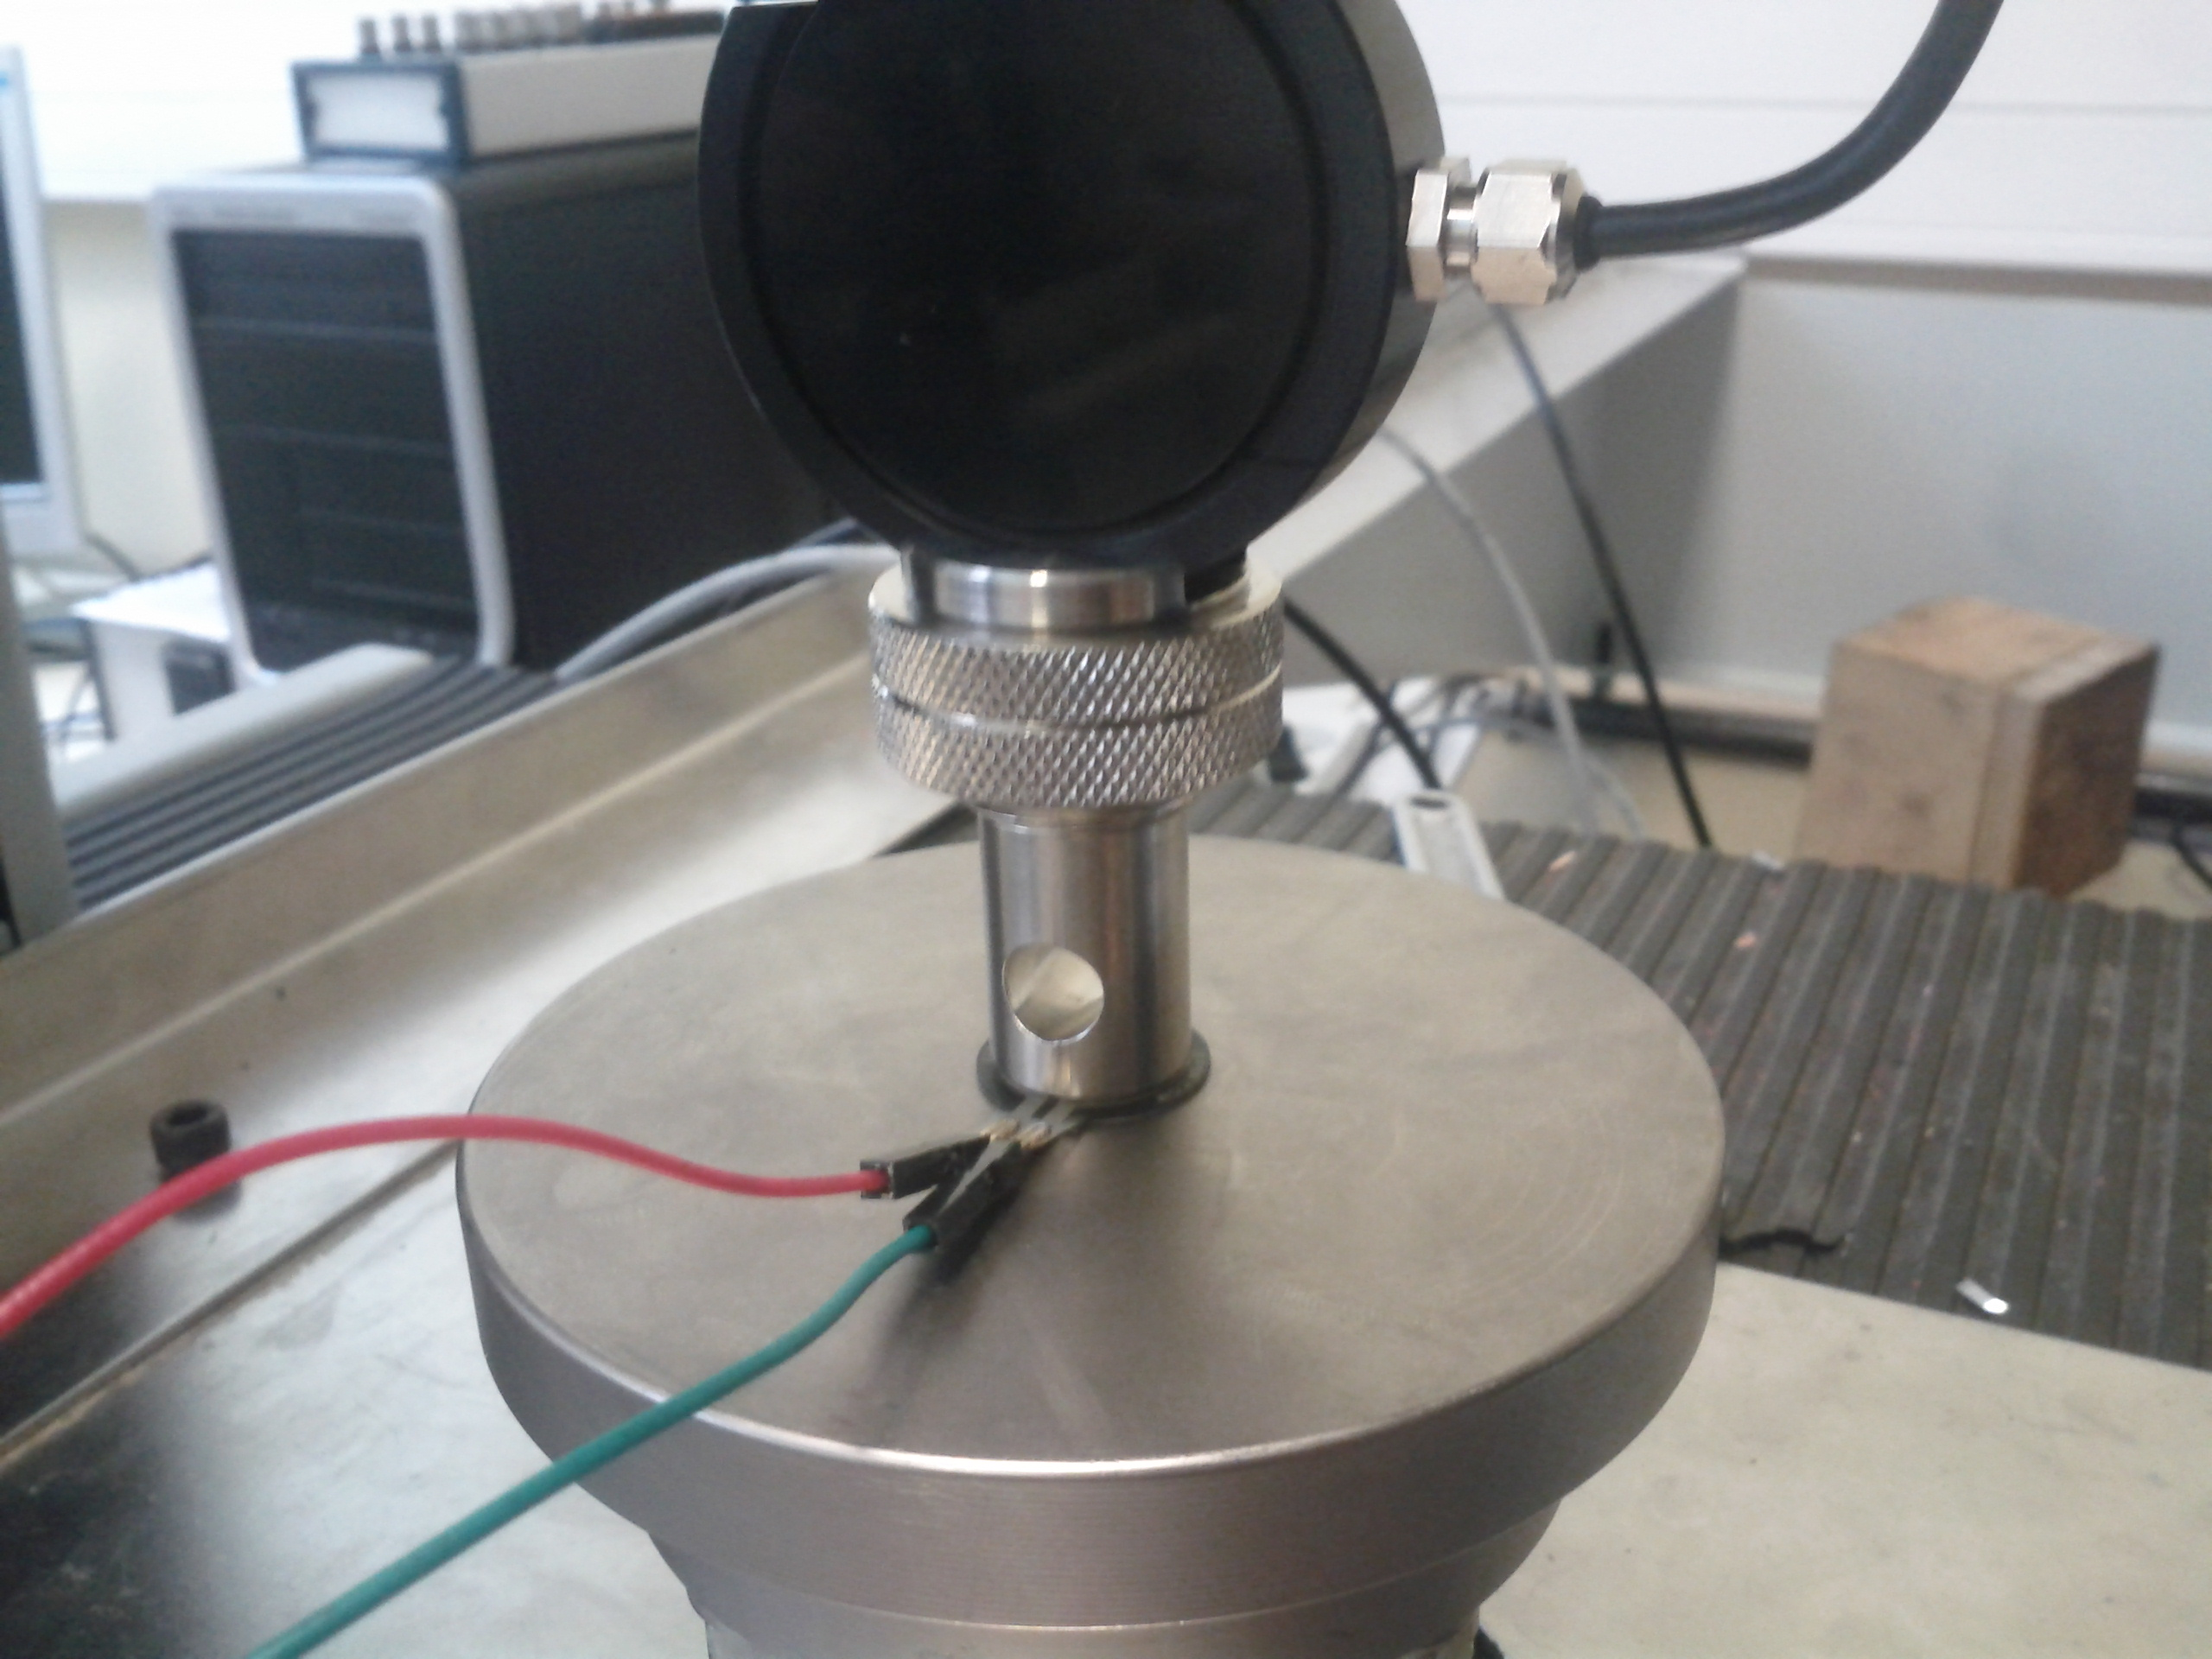
\includegraphics[scale=0.08]{testPression1.jpg}
		}
	\quad
	\subfigure{
		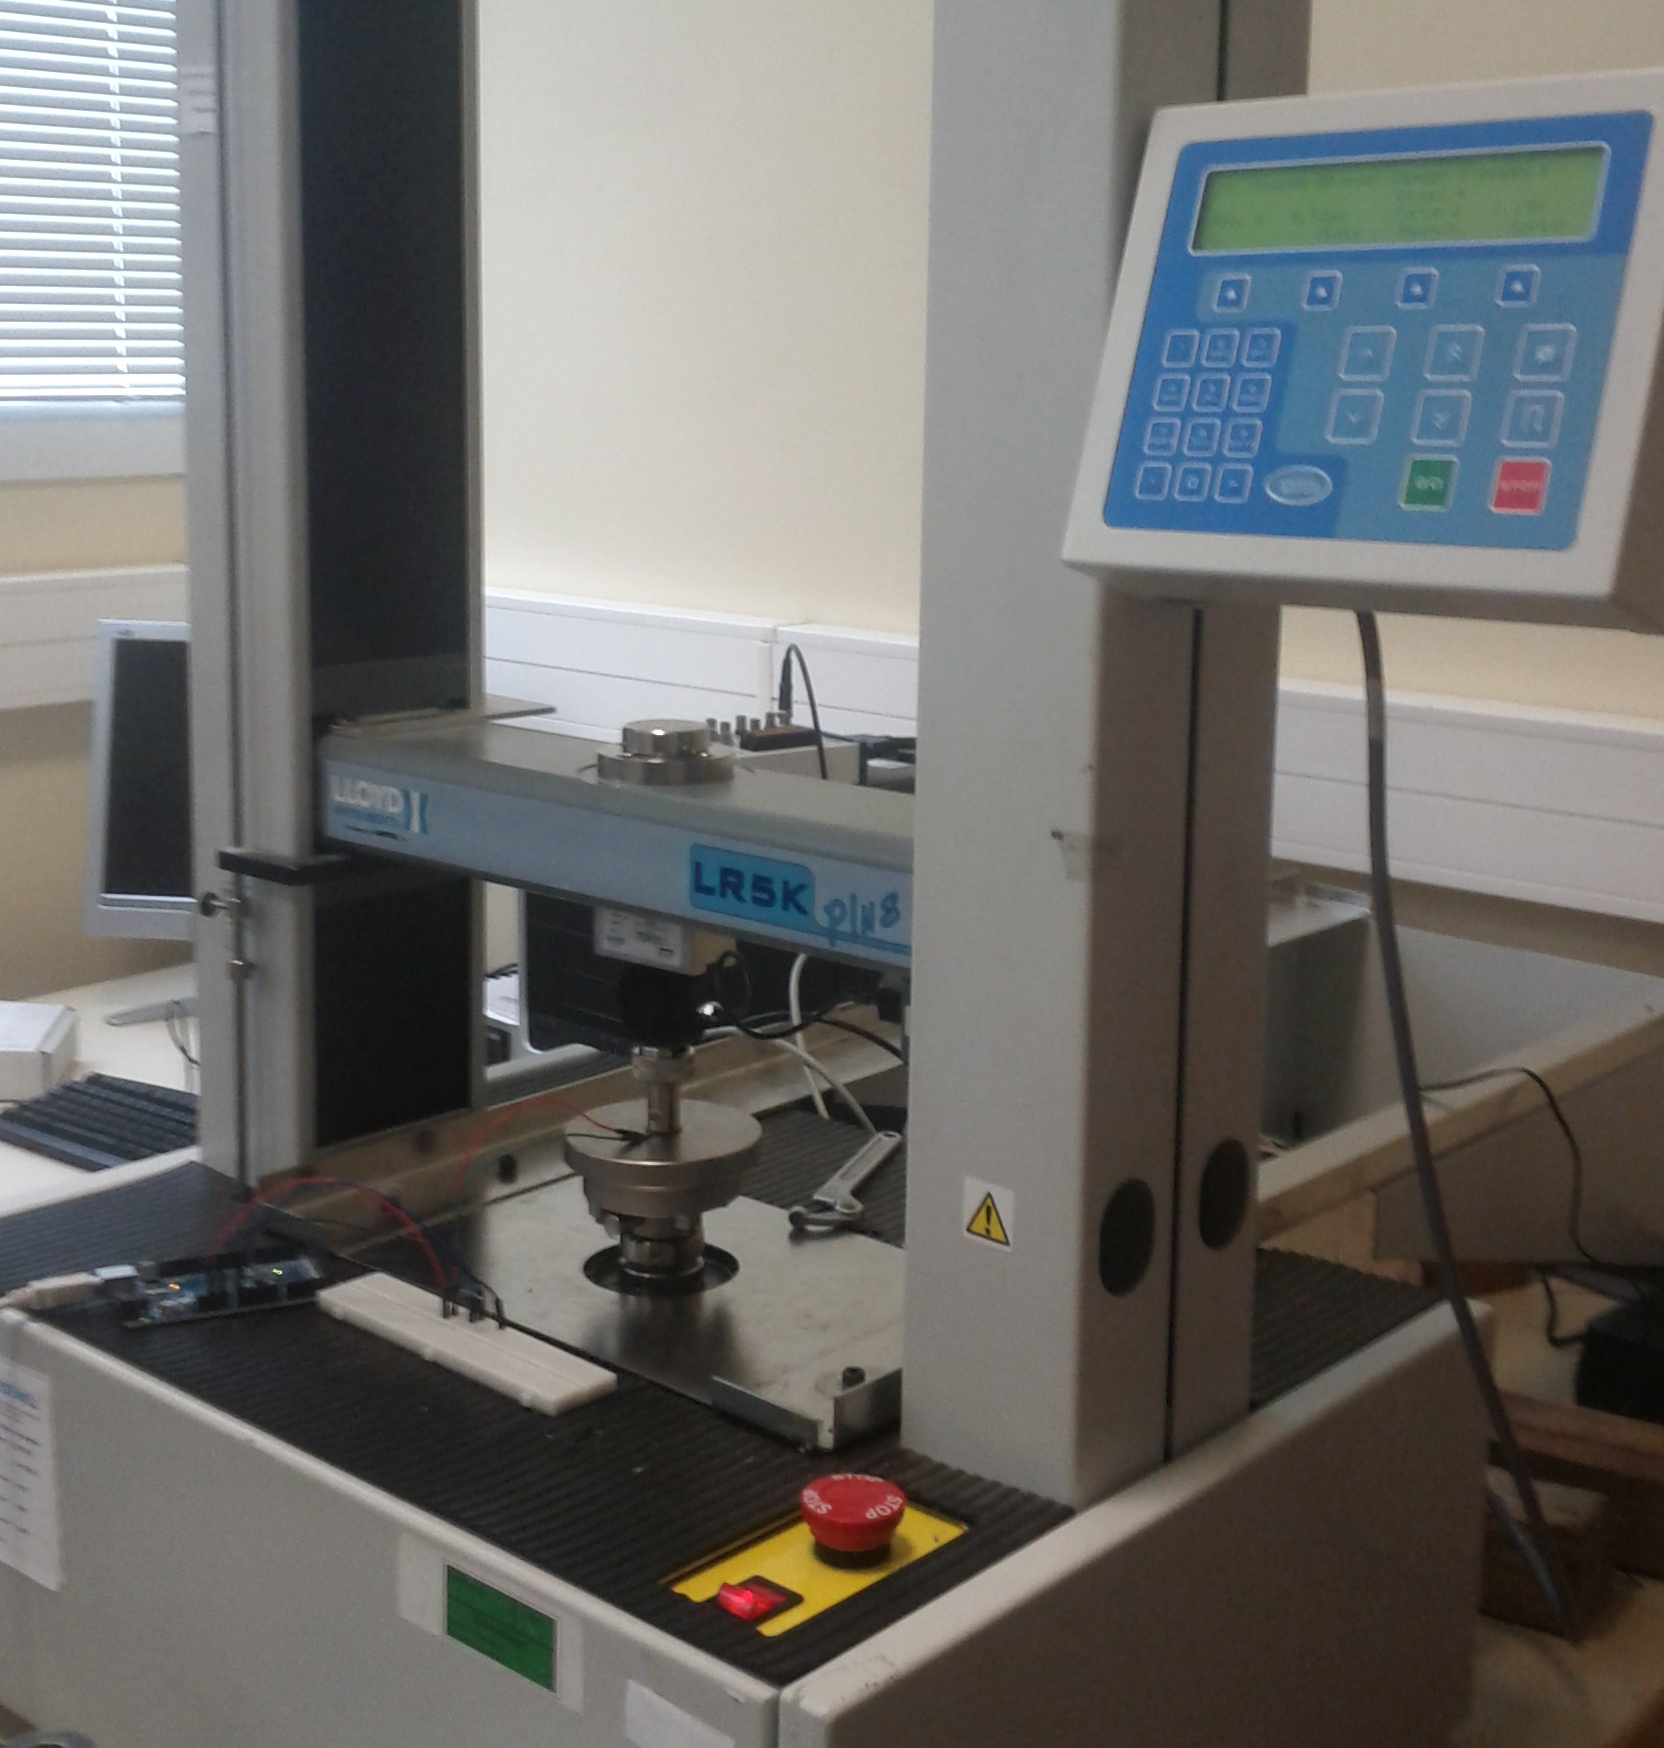
\includegraphics[scale=0.1]{testPression2.jpg}
		}
	\caption{\label{fig:pression} \'Etalonnage des capteurs de pression dans un laboratoire de mécanique de l'ENSTA Bretagne }
\end{figure}


L'ensemble des valeurs obtenues nous a permis de tracer la courbe qui nous donne une mesure de masse en fonction de la tension en sortie du capteur, voir figure \ref{fig:courbe}. Nous avons ensuite obtenu une équation de cette courbe de tendance. L'équation de cette courbe est de type polynomiale de degré 6 et $R²=0.96$. Comme les calculs de conversion ne seront pas effectués par l'Arduino mais par le serveur, la forme de cette équations n'est pas problématique. Nous avons également vérifié que tous les capteurs de pression suivent bien la même loi. Nous avons donc une formule unique de conversion de la tension de sortie en masse appliquée.

\begin{figure}[!h]
\centering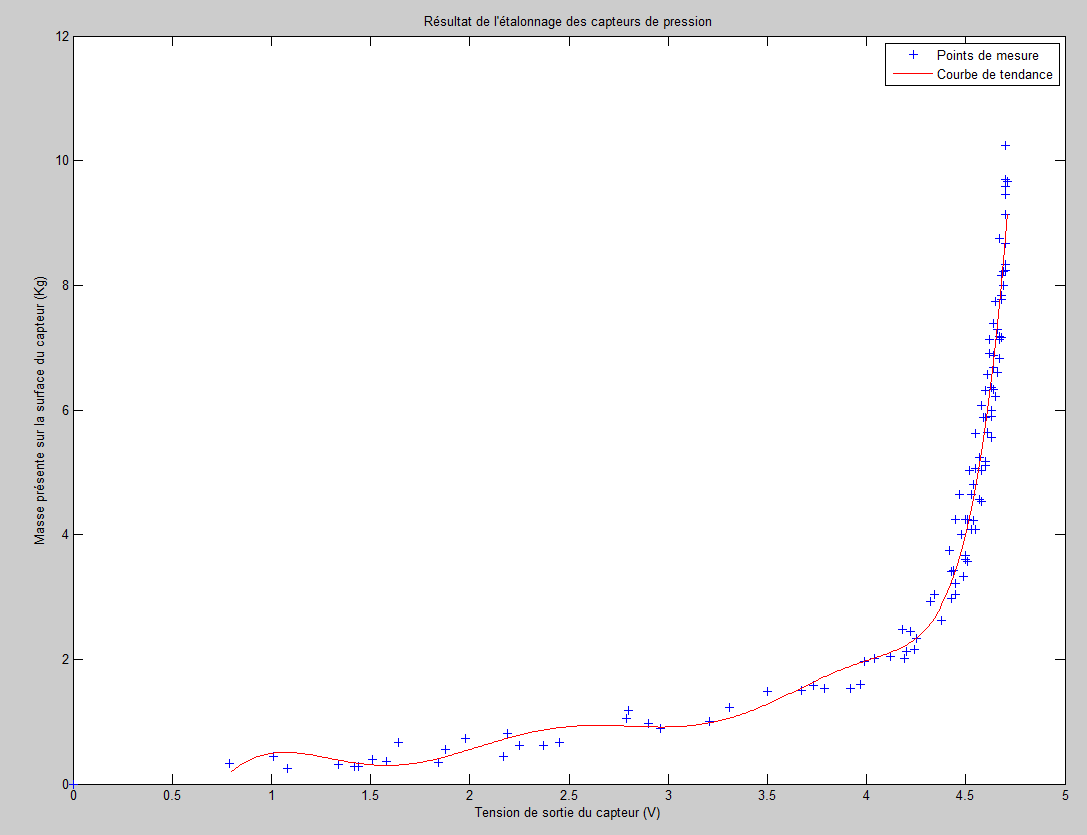
\includegraphics[scale=0.3]{courbe.png}
\caption{\label{fig:courbe} Courbe de tendance obtenue par l"étalonnage des capteurs de pression}
\end{figure} 

\section{Gestion des données par Arduino}